\hyperref[sec:sec7]{\section{香港人當年是否害怕九七?}}
\label{sec:sec6}

香港人害怕九七,但害怕的表達方式有很多種。表現得很快樂,也可以是為了埋藏心中的害怕。在一九八九至一九九七期間,香港人的身分認同出現了很多轉折,在極短時間來經歷了錯愕、拒絕、逃避,但在臨近九七的一兩年卻反過來對未來表現出可稱為不切實際的樂觀情緒。香港人在極短時間內表現得如此反覆,現在回頭來看並不代表香港人的身分認同本質上有很大改變,而是這個身分認同本身就相當複雜,看似自相矛盾的情感實為同一個銅幣的兩面。

一九八九年的北京民主運動,無論對中國大陸或是對香港來說都是一件分水嶺事件。北京民運的來龍去脈以及各方應該承擔的責任,已有很多專著論及,在此不贅。歷時近兩個月的運動以血腥鎮壓告終,對於中國大陸來說固然代表了八十年代以來的開放風氣被打斷,及後更因為中共處處提防而難以重返。對於香港來說,則基於香港社會於八九民運當中的全城參與,中國政府對港政策大幅調整,形成往後中港之間「收緊、反抗、打壓」的循環格局。

香港社會於八九民運當中的全城參與,可體現在很多不同層面。當時的電視新聞為了報道北京的消息,每天傍晚半小時的新聞時段基本上都是說北京的消息,以及香港各界的反應。其他的新聞都沒有時間說,連同體育消息一起推到晚上十一時的晚間新聞才播出。香港社會對民運的支持可謂完全一面倒,除了百萬人上街大遊行和在馬場連續舉行十二小時的「民主歌聲獻中華」之外,尚有很多今天意想不到的人物和團體表達支持,例如色情刊物《龍虎豹》也發動義賣支持北京學生。當北京宣布戒嚴翌日,親中報章《文匯報》於社論刊出「痛心疾首」四個大字,作「開天窗」式抗議。同期報章又常有各界刊登廣告表示支持北京學生,要求撤銷戒嚴和解除新聞封鎖,當中包括商界領袖如李嘉誠、何鴻燊、鄭裕彤、李兆基、郭炳江等,又有政界領袖如曾鈺成、唐英年、梁愛詩、田北俊和梁錦松,還有後來當上香港行政長官的梁振英。

\begin{figure}[htbp]
    \centering
    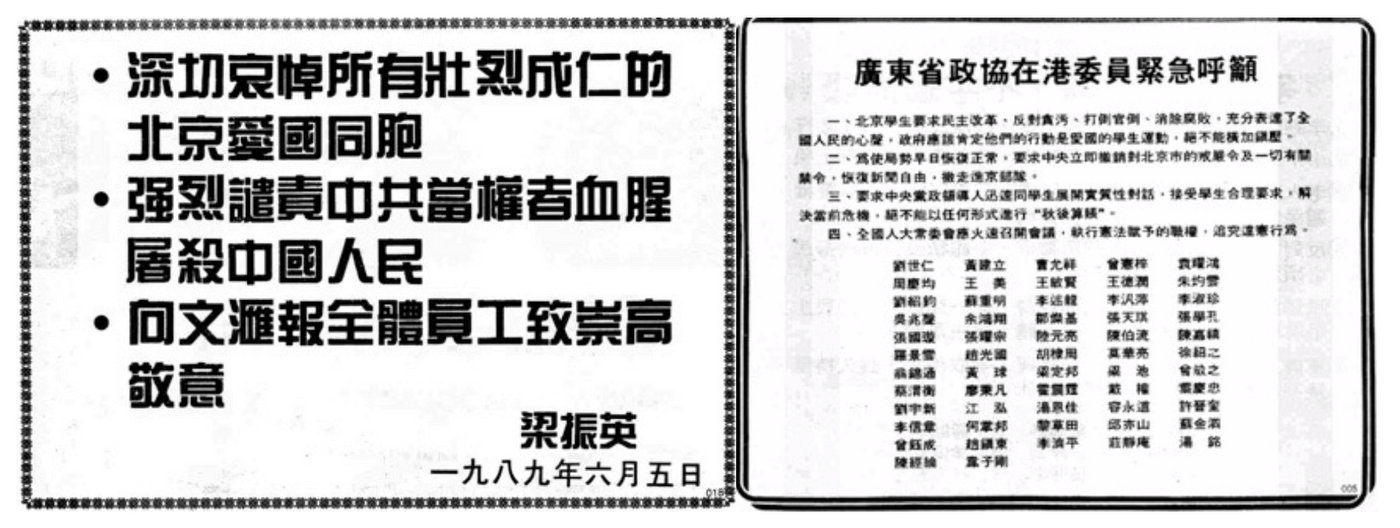
\includegraphics[width=0.7\textwidth]{c06/condolences.png}
    \caption{香港報章刊登聲援八九民運的廣告} 
\end{figure}

到了民運後期,香港各界成立了「香港市民支援愛國民主運動聯合會」(簡稱支聯會)來組織支持民運的行動,這個組織後來成為了每年主辦六四燭光悼念集會的主辦者。支聯會的名字包括「愛國」和「民主」,以這兩個詞語來總結香港人對北京民運的關注和支持可謂十分準確。首先,雖然八九民運以民主為題,但當時的香港並不見得十分民主,香港人普遍的民主認知其實十分有限。當年立法局尚未設有直選議席,僅有的民主選舉只限於區議會和市政局,而且投票率也不高。如果說當時的香港人要把民主帶到中國,未免有點說不過去。

但把「民主」和「愛國」放在一起,對當時的參與者來說就彷佛合理得多。面對「九七大限」尚餘八年,「要做一個怎樣的中國人」是香港人必須回答的問題。讓香港變得和中國大陸沒有分別固然不能接受,如果要有中港融合的話也應該是中國大陸變得更像香港,而不是相反。前文提到《這是我家》帶出香港可以通過橋樑角色來在中國之內保持獨特身分,香港人對民運的支持便成為了這個角色的一種體現:支援北京學生(無論是精神上還是資源上)其實是一種港式愛國行為,代表了香港人要以一種獨特身分來處身中國和貢獻中國。當時民運中就出現了大量的愛國措辭,遊行集會當中也常聽到《龍的傳人》等的愛國歌曲。與此同時,當時大多數的香港人也相信中國政體的民主化,也相信它對保護未來一國兩制下的香港獨特性肯定有利。

可以想像,在全港市民包括權貴階層和親中陣營都支持八九民運的背景下,當北京武力鎮壓的消息傳來香港的時候,帶來的震撼固然是巨大無比。但在鎮壓當晚,也看到香港人在當時整個中國想像當中的特殊地位。不同的現場紀錄都訴說同一個情況:北京市民冒險保護現場的香港學生和記者,甚至不惜以血肉之軀在槍林彈雨下作掩護,好讓他們能安全離開,把鎮壓的消息帶出中國。香港在中國的邊緣位置,對當時的北京市民來說是至關重要和得務必珍惜的。

% \begin{figure}[ht!]
%     \centering
%     \includemedia[
%     width=0.6\linewidth,height=0.45\linewidth,
%     activate=pageopen,
%     flashvars={
%         modestbranding=1  % no YT logo in control bar
%         &autohide=1       % controlbar autohide
%         &showinfo=0       % no title and other info before start
%     }
%     ]{}{https://youtu.be/C3no_C6v2yI}   % Flash file
%     \caption{六四鎮壓特別新聞報道}
% \end{figure}

往後兩三年的時間,整個香港社會都被悲憤所壓抑,同時對不久之後便要來臨的「九七大限」無比恐懼。畢竟,對於很多香港人來說,他們或他們的父母前來香港,就是為了脫離中國大陸的政治動盪;八九民運卻提醒他們,即將在九七接管香港的那個政府和當年他們所脫離的,其實是同一個中國政府。

正正在這個時候,香港出現了大量以搞笑為主題的文化產品。例如今天已是一代諧星的曾志偉和林敏聰,就在一九九零年和一九九一年於亞洲電視製作了搞笑節目《開心主流派》,而同期無綫電視則以《笑星救地球》迎戰,帶動「無厘頭文化」。香港棟篤笑始祖黃子華,也在一九九零年舉辦首場棟篤笑演出。至於香港喜劇殿堂級代表周星馳,其早期代表作品如《賭聖》和《逃學威龍》的上映時間,同樣是一九九零年和一九九一年。在這段時間,香港人太需要笑,因為香港人太想哭。

搞笑的方法可以有很多種,而這段時間不少的搞笑情節都和中港關係相關,特別是對中國政治的各種諷刺,成為了香港人抒發不滿和恐懼的重要方式。一九九零年上映的電影《表姐,你好嘢!》可謂當時政治諷刺的經典之作,片中由鄭裕玲飾演的中國女公安來到香港協助查案,因為不懂得香港的法治和人權制度而弄出許多衝突。此外,一九九四年上映的的電影《國產凌凌漆》,也把中國大陸各種貪污腐敗用作為搞笑橋段。故事描述周星馳飾演的中國特務前來香港調查恐龍化石被盗,然而他的上司才是幕後黑手。其中一幕周星馳幾乎被鎗決,卻能靠一百元收買處決小隊脫身,此橋段後來常被借用評論中國政治。

說到電影中的中國想像,同期電影中經常出現來自中國大陸的特異功能人士,如《賭聖》和《賭俠》系列中的左頌星/周星祖和大軍,以及《表姐,妳好嘢!》中的阿勝。這和同期中國大陸流行的超能力風潮(如張寶勝)相對應,但也乎合了當時香港人感到中國神秘和變幻莫測。與此同時,又有大量描述中國大陸悍匪的電影,如《省港旗兵》系列,背景既和當時相當猖獗的跨境犯罪搶劫有關,也反映出社會感到來自中國大陸各方面的威脅。此系列到了第四集時,更直接挪用八九民運作為劇情主軸。

除了以搞笑或直接描述外,當年還有不少影視產品以各種隱喻方式回應歷史巨變。一九九零年電影《倩女幽魂2之人間道》,就被認為是香港影視界回答八九民運的經典,監製徐克後來坦言片中角色都有影射中國領導人、民運學生,和香港人。而片中由黃霑作曲和填詞,張學友主唱的主題曲,更明言「少年怒/天地鬼哭神號」和「大地舊日江山/為什麼變成了血海滔滔/故園路怎麼盡是不歸路/驚問世間怎麼盡是無道」,後來黃霑也公開承認此曲實以八九民運為題。此曲後來於八九民運三十週年前夕在中國大陸忽然被禁。

面對難以改變的現實,說笑話或以影射來舒解恐懼很大程度上只是精神逃避。要從現實上逃避中國管治,只有移民一逃。從一九九零年到一九九四年期間,有超過三十萬香港人移民外地,當中大多數以英國、加拿大、澳洲和美國為目的地,在當地建立起新的香港人社區,如溫哥華就有 “Van Kong” 一說。當時香港人移民海外的普遍程度,使得移民成為了電視劇集中情侶分手的最合理解釋。移民現象也成為了社會批判的一個窗口,例如李克勤的歌曲《後會有期》雖然表面上是一首情歌,然而當中「誰在這邊趕上機/誰在那邊講道理/害怕等最後限期像處死」的歌詞卻明顯是在控訴當時有從政者一方面高呼愛國愛港,同時安排家人取得外國護照的矛盾行為。

% \begin{figure}[ht!]
%     \centering
%     \includemedia[
%     width=0.6\linewidth,height=0.45\linewidth,
%     activate=pageopen,
%     flashvars={
%         modestbranding=1  % no YT logo in control bar
%         &autohide=1       % controlbar autohide
%         &showinfo=0       % no title and other info before start
%     }
%     ]{}{https://youtu.be/dRgnbwT_EDY}   % Flash file
%     \caption{《後會有期》1991 主唱李克勤 填詞Pace Lumba}
% \end{figure}

順帶一提,有意見認為這段移民潮為香港的中上層製做了一個奇怪的斷層:最有能力的老前輩紛紛離開,中層人員儘管歷練不足卻因而有機會快速晉升,然後這一代人霸佔管理層三十年之久,引發社會世代流動不暢。對他們來說,他們的快速晉升加強了他們對香港充滿機會,若有人失敗只可能是個人問題的盲目崇拜;而由於他們本身能力不足,才引至後來香港各方面的逐漸敗壞。這種說法從學究上來說未免過於簡化,但類似說法既然能夠流行起來,也反映出社會對移民潮和世代矛盾的一種理解。

當然,並不是所有香港人都有能力移民,可以離開的往往都以中產專業為主。這個階級分野也受到官方政策的強化。當時曾有本地政治代表向英國政府要求向全港五百多萬市民提供「居英權」,一方面顯示英國對香港前途有信心,也對擔心前途的香港人給予一個最後出路。礙於擔心香港人都會湧往英國定居,最終英國政府只提供了五萬名的名額,容許擁有特殊專業技能的專業人士、企業家商人、紀律部隊公務員,以及從事敏感工作職位(例如警察政治部)的人士申請。面對中產專業紛紛離開香港,當時社會也流行說:「有錢有辦法,無錢基本法」,諷刺港人只是在沒有選擇的情況下接受主權移交。

對於中國大陸的當權者來說,香港市民對八九民運的支持則帶來另一個難題。八九民運本來到了中後段有無以為繼的趨勢,卻在來自北京以外的支持下繼續下去,當中來自香港的精神支持和實際物資有顯著影響。僅是「民主歌聲獻中華」的活動,就籌得一千三百萬港元的捐款。香港專上學生聯會直接送了數十個色彩鮮艷的野營帳篷到天安門廣場,也讓廣場上的人精神一振。到了鎮壓以後,以香港為基地的「黃雀行動」又協助營救了數以百計的民運領袖離開中國。這些實際的影響,使當權者擔心香港將會變成「反共基地」。畢竟,當年孫中山推翻滿清就是從香港開始,香港自開埠以來其存在就是對中央集權的一個挑戰。江澤民於八九年年底會見英國首相特使的時候就提到「井水不犯河水,河水不犯井水」的說法,意謂香港人不應干涉中國大陸政治。以後中國政府處理香港民主化的問題時,也必先考慮到與中共管治的相互影響。而當時正在草擬當中的香港《基本法》,不少條文的定稿方案也比原先的諮詢稿有明顯的收緊,特別是與選舉方式和國家安全相關的條文。

中國政府對香港民主化的擔憂,很快就放上政治議程。面對六四鎮壓,英國作為一個民主國家,也要處理如何向選民交待要將香港交予中國統治。英國政府的答案,是要加速香港的民主化,盡可能在一九九七年前為香港建立一個民主制度,以防未來北京可能對一國兩制所作的干擾。畢竟,《中英聯合聲明》已規定了港人治港,港英政府以此為基礎擴充香港的民主化,他們認為既能對香港人和國際社會交代,也不應被視為背叛對北京的承諾。與此同時,香港人本身也要求加速香港的民主化,作為主體移交後香港自主的保障,也就是所謂的「民主抗共」。

港英政府具體的民主化措施,體現在一九九二年就任香港總督的彭定康所提出的政治改革方案。全國人民代表大會已於一九九零年決定了香港特區第一屆立法會的組成方法,並列明原香港最後一屆立法局可留任成為第一屆立法會的議員,也就是所謂的順利過渡和「直通車」。方法規定六十個議席當中有三十席由功能團體選舉產生,而一九九一年產生的立法局只有二十一個議席由功能團體選舉產生,所以一九九五年的選舉要新增九個功能團體席位。本來功能團體席位通常由商界領袖所主導,彭定康卻想到把所有選民按職業分為九組(當時稱為「新九組」),讓所有選民都能夠成為功能組別選民,變相把這九席等同直選。這做法大幅提高了立法局的代表性,但從中方的角度出發卻等於是港英政府強行改變了第一屆立法會的組成方法。如是者,中英兩國的政改爭拗就此展開,英方說「三乎合」(乎合《中英聯合聲明》等協議),中方則說「三違反」,兩邊互罵無日無之。

與此同時,中英雙方又就香港的新機場計劃展開爭拗。香港的國際機場原設於九龍城,隨城市發展已被建築物包圍,無法擴建,大大限制了香港的國際連結,必須另建新機場。港英政府在六四鎮壓後為顯示對香港未來的信心,推出香港史上最大規模的基建發展計劃,除了新機場外還有機場高速公路和鐵路綫,全球最長的公路鐵路兩用大橋,以及鐵路沿線的城市發展,合稱之為「玫瑰園計劃」。中方對此卻十分擔心,懷疑港英政府刻意要在一九九七年之前把政府的儲備全數花光,於是兩國又就機場計劃展開談判。

政改爭拗最後以「另起爐灶」結束,中方不承認一九九五年的選舉方案,另行成立「臨時立法會」於一九九七年接手,一九九五年選出的立法局議員不能自動成為特區的第一屆立法會議員。新機場協議經多翻修訂,最終位於赤鱲角的新機場在一九九八年啟用,港英政府也為特區留下三千億元儲備,遠比協議規定的二百五十億為多。不過,在這些關係到香港前途的談判當中,香港人無從參與,香港記者往往只能在多次閉門會議的前後探取風聲,透過兩國代表的片言隻語來捕風捉影。對此,不少香港人對無法掌握自己的未來感到越來越不滿。

從中英談判和一九八四年《中英聯合聲明》的草議開始,香港人就被排除在決定香港命運的過程當中。香港革新會在一九八二年的民意調查就顯示由七成市民希望香港在一九九七年後維持為英國殖民地,一成半的市民支持改由聯合國託管,只有百分之四的市民支持被中國收回並受中國管治。一九八三年時又有簽名運動,多達六十三萬個簽名支持維持現狀。這些數據和中國官方傳媒經常宣稱的「香港同胞熱切期望回到祖國懷抱」的說法,可謂差天共地。本來「一國兩制」的設立是為了釋除香港人對中國管治的疑慮,但談判過程卻沒有港方的參與,中方堅持只和英方直接對話。當時香港輿論有所謂「三腳櫈」的說法,即談判過程要有中、英、港三方的參與才能穩健。然而鄧小平在一九八四年會見香港的議員代表時,劈頭就說:「所謂三腳凳,沒有三腳,只有兩腳」。再看同期香港觀察社的民調,百分之九十五的市民應為香港人應該有份決定香港前途,其中專上教育程度者更是百分之一百認同,可見訴求之廣和落差之大。

九十年代初新一波的中英爭拗,再次突顯了香港人對自身前途的無力感。而經歷過八九民運的洗禮,不少人對於政治參與變得更為進取,認為要讓香港人自己發聲,也有所謂「夾縫論」的出現,主張香港人不應再被動地為「英國殖民主義者或中國權威主義」所戲弄(周蕾)。類似的訴求在流行文化中也有出現,如樂隊 Beyond 《爸爸媽媽》一曲當中,就把中英兩國爭拗理解為父母爭吵,然而香港這個孩子其實已經長大,可以決定自己的前途:
    爸爸要爭論昨日是誰錯 媽媽她心裡一把火
    乖乖已長大莫問是誰錯 只想你一句講清楚

    過渡期裡 戰鬥未曾過去
    我被遺棄 太過令人費解

    爸爸他說媽媽真失敗 今天真正主角是我嗎
    爸爸請你歸家休息吧 今天真正主角是我嗎
\begin{displayquote}
        爸爸要爭論昨日是誰錯 媽媽她心裡一把火
    乖乖已長大莫問是誰錯 只想你一句講清楚

    過渡期裡 戰鬥未曾過去
    我被遺棄 太過令人費解

    爸爸他說媽媽真失敗 今天真正主角是我嗎
    爸爸請你歸家休息吧 今天真正主角是我嗎
\end{displayquote}

% \begin{figure}[ht!]
%     \centering
%     \includemedia[
%     width=0.6\linewidth,height=0.45\linewidth,
%     activate=pageopen,
%     flashvars={
%         modestbranding=1  % no YT logo in control bar
%         &autohide=1       % controlbar autohide
%         &showinfo=0       % no title and other info before start
%     }
%     ]{}{https://youtu.be/Dhxe-m0PBuw}   % Flash file
%     \caption{《爸爸媽媽》 1993 主唱 Beyond 填詞黃貫中}
% \end{figure}

到了學術界,「夾縫論」的出現卻引來不少批評。有學者雖然認同其表達的不滿,卻同時認為背後的分析很容易把香港本質化,不利於香港社會反省自身的不足。例如當香港人要高舉資本主義來對抗當時中國大陸的社會主義時,便會忽視了香港經濟制度中的一些弱點,如對勞工保障的不足。學者孔誥烽當時就直指「夾縫想像」的問題在於「構作(/強化)了一個資本主義、中西混雜兼容並包、安定繁榮、有民主、有自由、有法治、有人權的『香港』自我;同時也構作了一個心胸狹窄、驕傲自大、社會主義的『中原文化』他者」,卻絕口不提「近年港商大舉北上,大陸的勞工、天然資源、市場甚理女性全成為他們的剝削對像」,未免與香港人的夾縫冤屈描述格格不入。因此,相對於把香港的問題簡化為中英兩國欺負香港,應該說是海外、國內以及本地的權貴階層利用轉變的時機大撈一筆,受害的實是各處的低下階層。

不過,這些討論很大程度上只停留在學術界當中。實際上越靠近九七,主流社會中的悲觀情緒便很快被另一種近乎盲目樂觀的表現所蓋過。但這不是說當時的香港人不再憂慮,反而更像是在沒有其他出路的前題下,選擇幻想明天必定會更好,作最後的自我陶醉。


伸延閱讀:

史文鴻(1993):〈近年港產片中大陸人的典型化問題〉,史文鴻、吳俊雄編《香港普及文化研究》,香港:三聯書店(香港)有限公司

孔誥烽(1997):〈初探北進殖民主義:從梁鳳儀現象看香港夾縫論)〉,陳清橋編《文化想像與意識形態:當代香港文化政治論評》,香港:牛津大學出版社。

吳俊雄(2002):〈尋找香港本土意識〉,吳俊雄、張志偉編《閱讀香港普及文化》,香港:牛津大學出版社。